\documentclass[10pt,aspectratio=43]{beamer}

\usepackage{graphicx}
\usepackage{tikz}
\usepackage{xcolor}
\usepackage{caption}
\usepackage{subcaption}
\usepackage{bm}
\usetikzlibrary{calc} 
\usepackage{hyperref}
\hypersetup{
    colorlinks=true,
    linkcolor=blue,
    urlcolor=red
}
\usepackage{fontawesome5}
\usepackage{ulem}
\usepackage[dvipsnames]{xcolor}

\usetheme{MyStyle}   % loads beamerthemeMyStyle.sty
\setlength{\columnsep}{0pt}


%%%%%%%%%%%%%%%%%%%%%%%%%%%%%%%%%%%%%%%%%%
%%%%%%%%%%%%%%%%%%%%%%%%%%%%%%%%%%%%%%%%%%
%%%%%%%%%%%%%%%%%%%%%%%%%%%%%%%%%%%%%%%%%%

\title{Fix bugs about some wfType 2 incorrectly classified as 4}
\newcommand{\eventname}{ALERT meeting}
\author{Felix Touchte Codjo}
\institute{IJCLab}
\date{November 2, 2026}


\begin{document}

\begin{frame}[plain] % remove header, footer, barre de navigation
\titlepage
\end{frame}

%\begin{frame}{Outline}
%\tableofcontents
%\end{frame}

%\section{Intro}
\section{Updates}


\begin{frame}{Bug: Waveform type 2 classified as 4}
    \begin{itemize}
        \item \textbf{Bug:} some wfType 2 (missing trailing edge) were classified as 4 (bad ToT, noise) because their ToT were below 300 ns
        %\item 
        
    \end{itemize}

    \centering
    \vspace{0.2cm}

    \begin{minipage}{0.35\linewidth}
        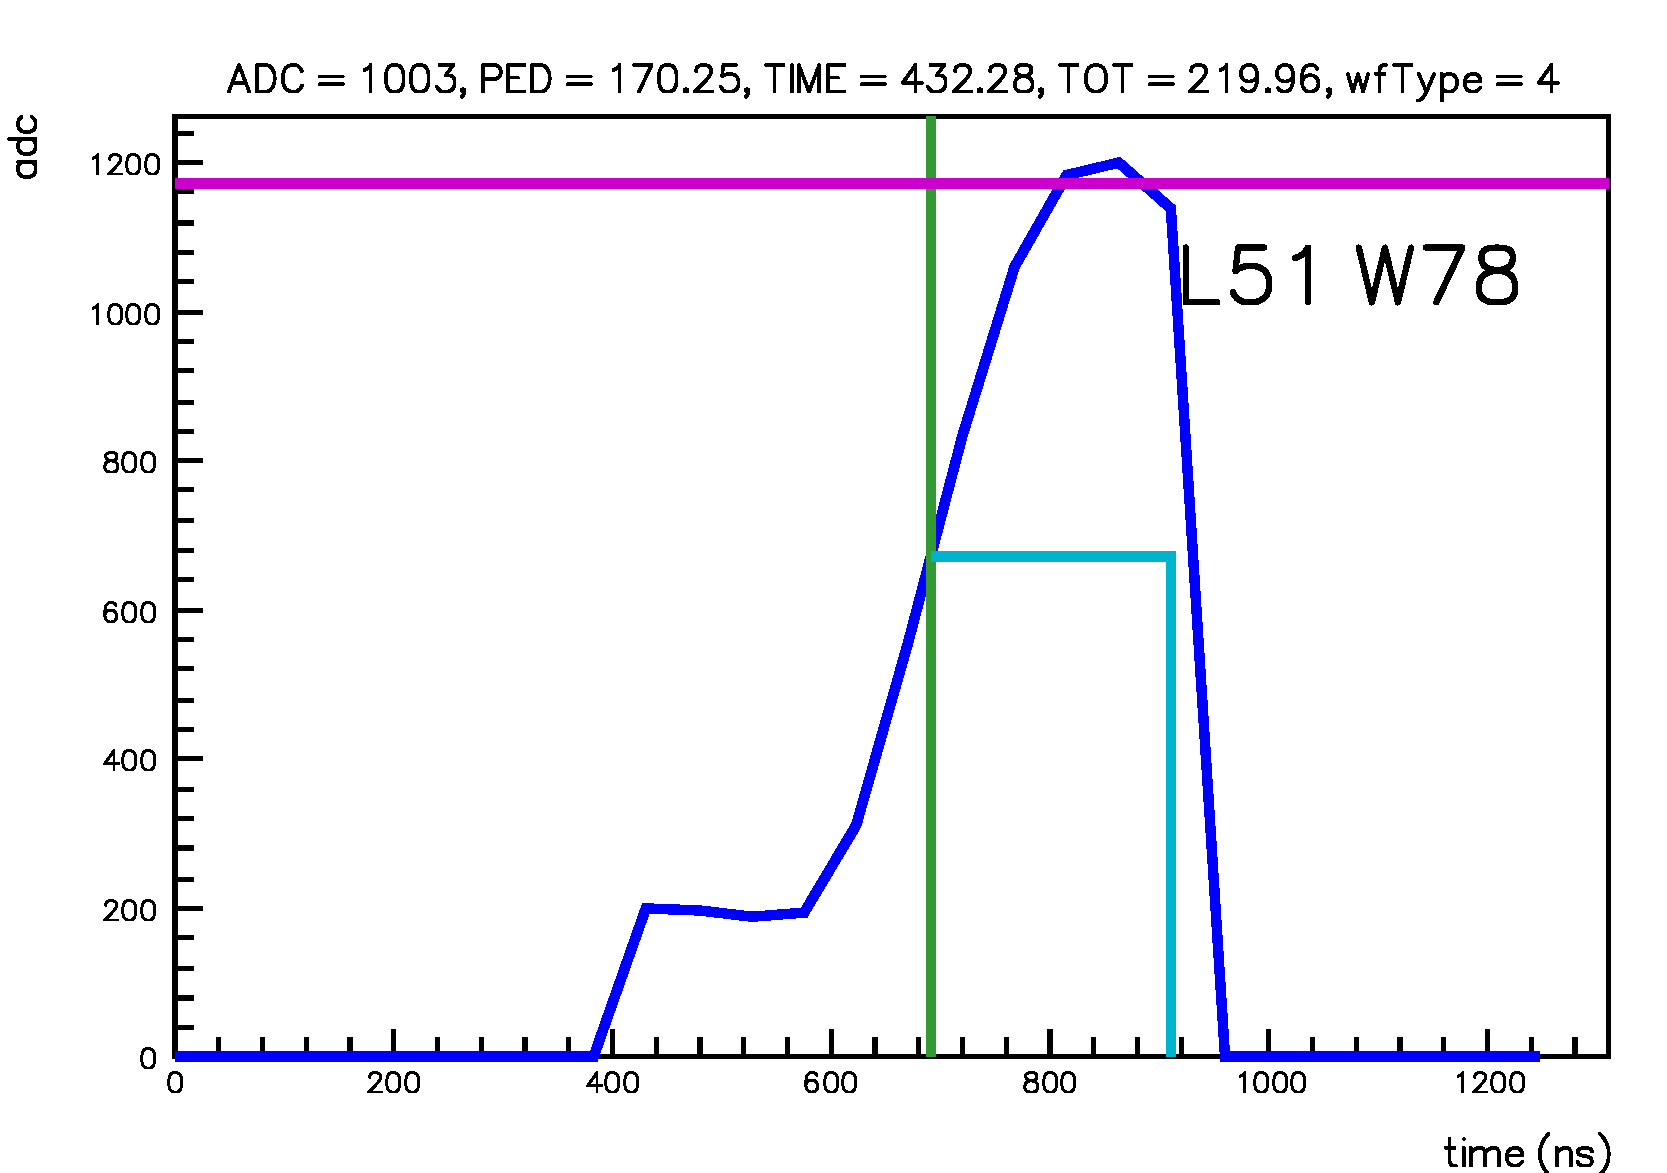
\includegraphics[width=\linewidth]{figures/wf1_before.pdf}
        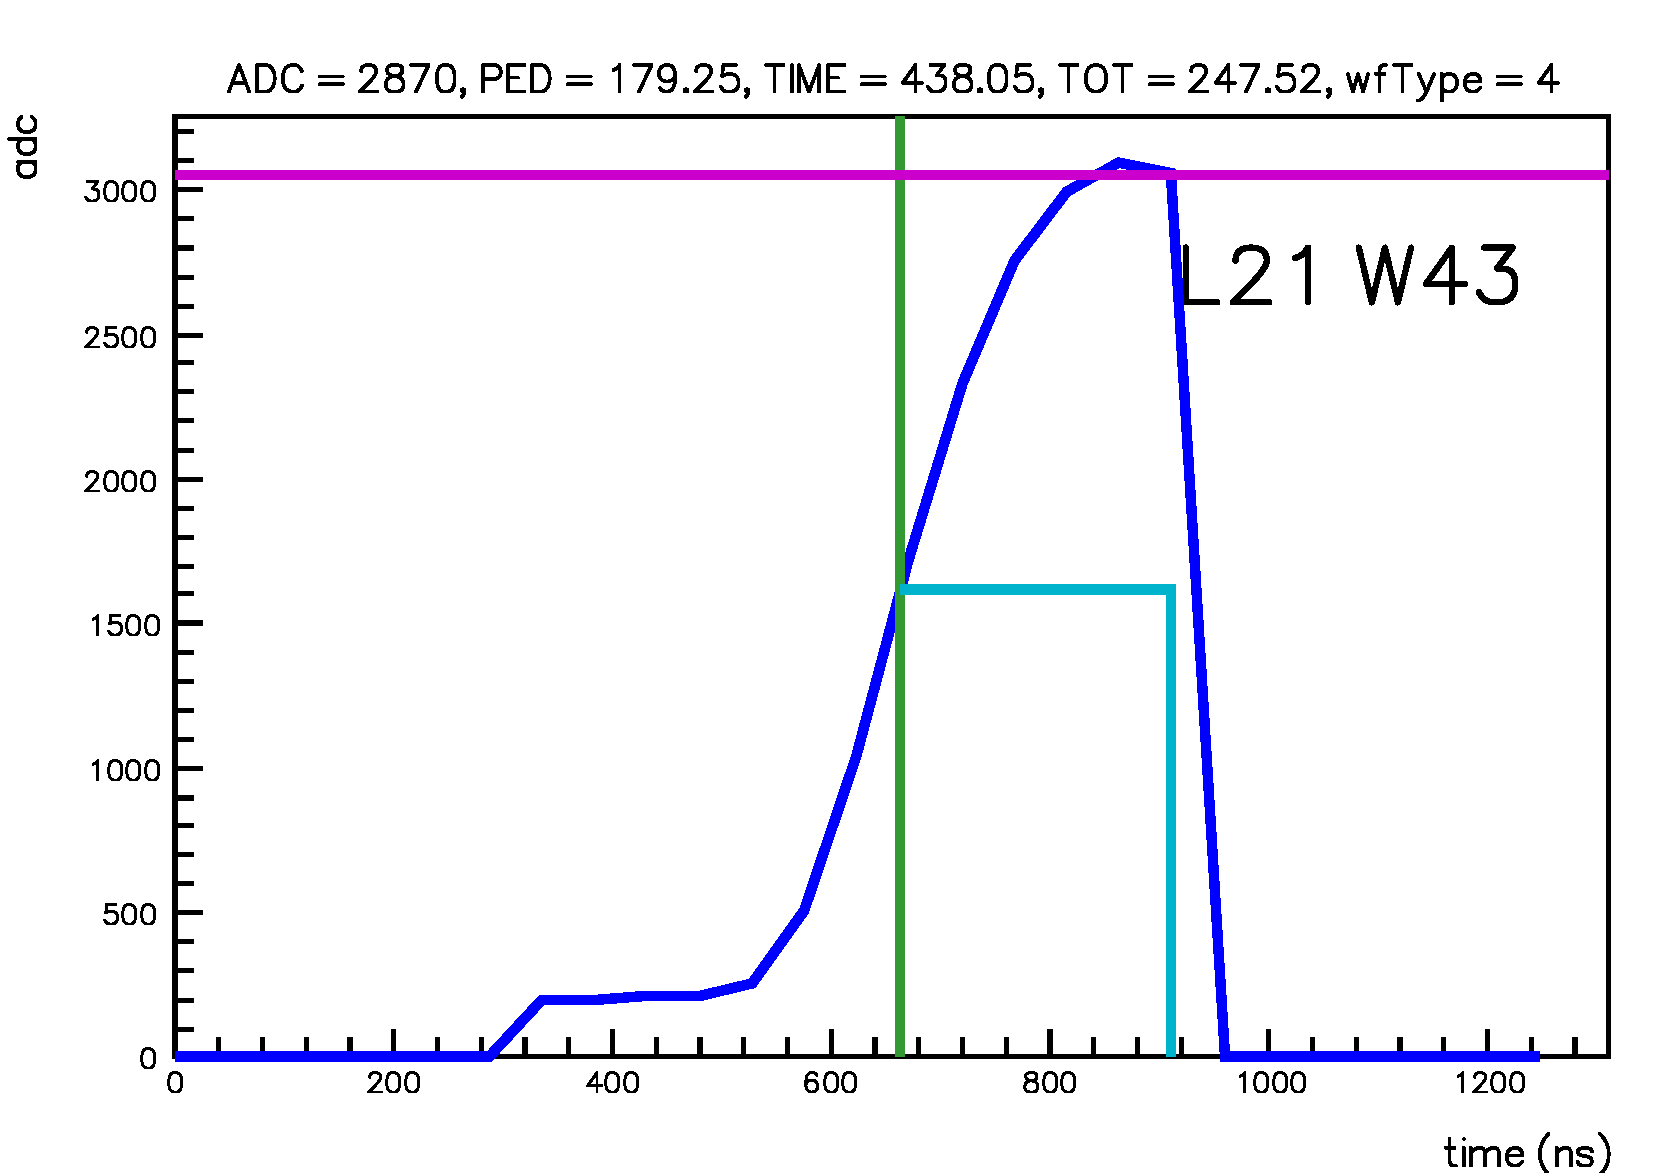
\includegraphics[width=\linewidth]{figures/wf2_before.pdf}

        \centering
        {\color{red} Before}
    \end{minipage}
    \hspace{0.3cm}
    \begin{minipage}{0.35\linewidth}
        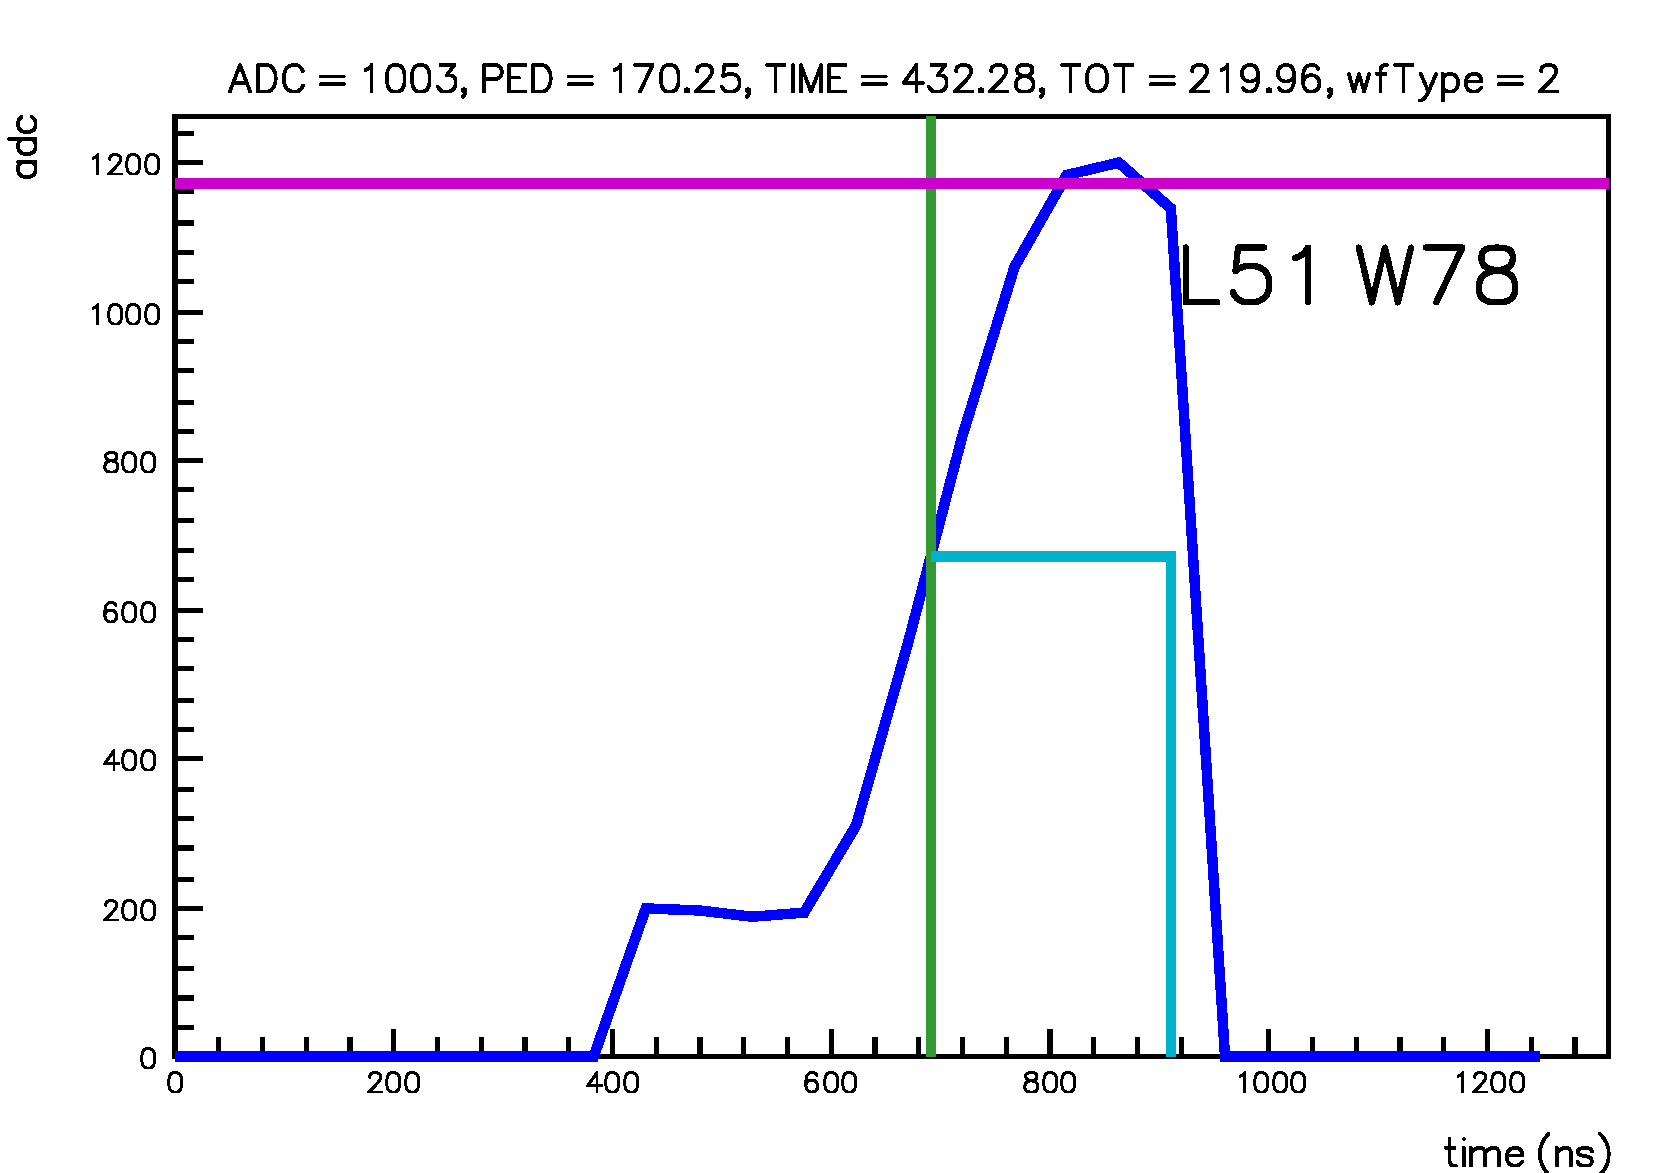
\includegraphics[width=\linewidth]{figures/wf1_after.pdf}
        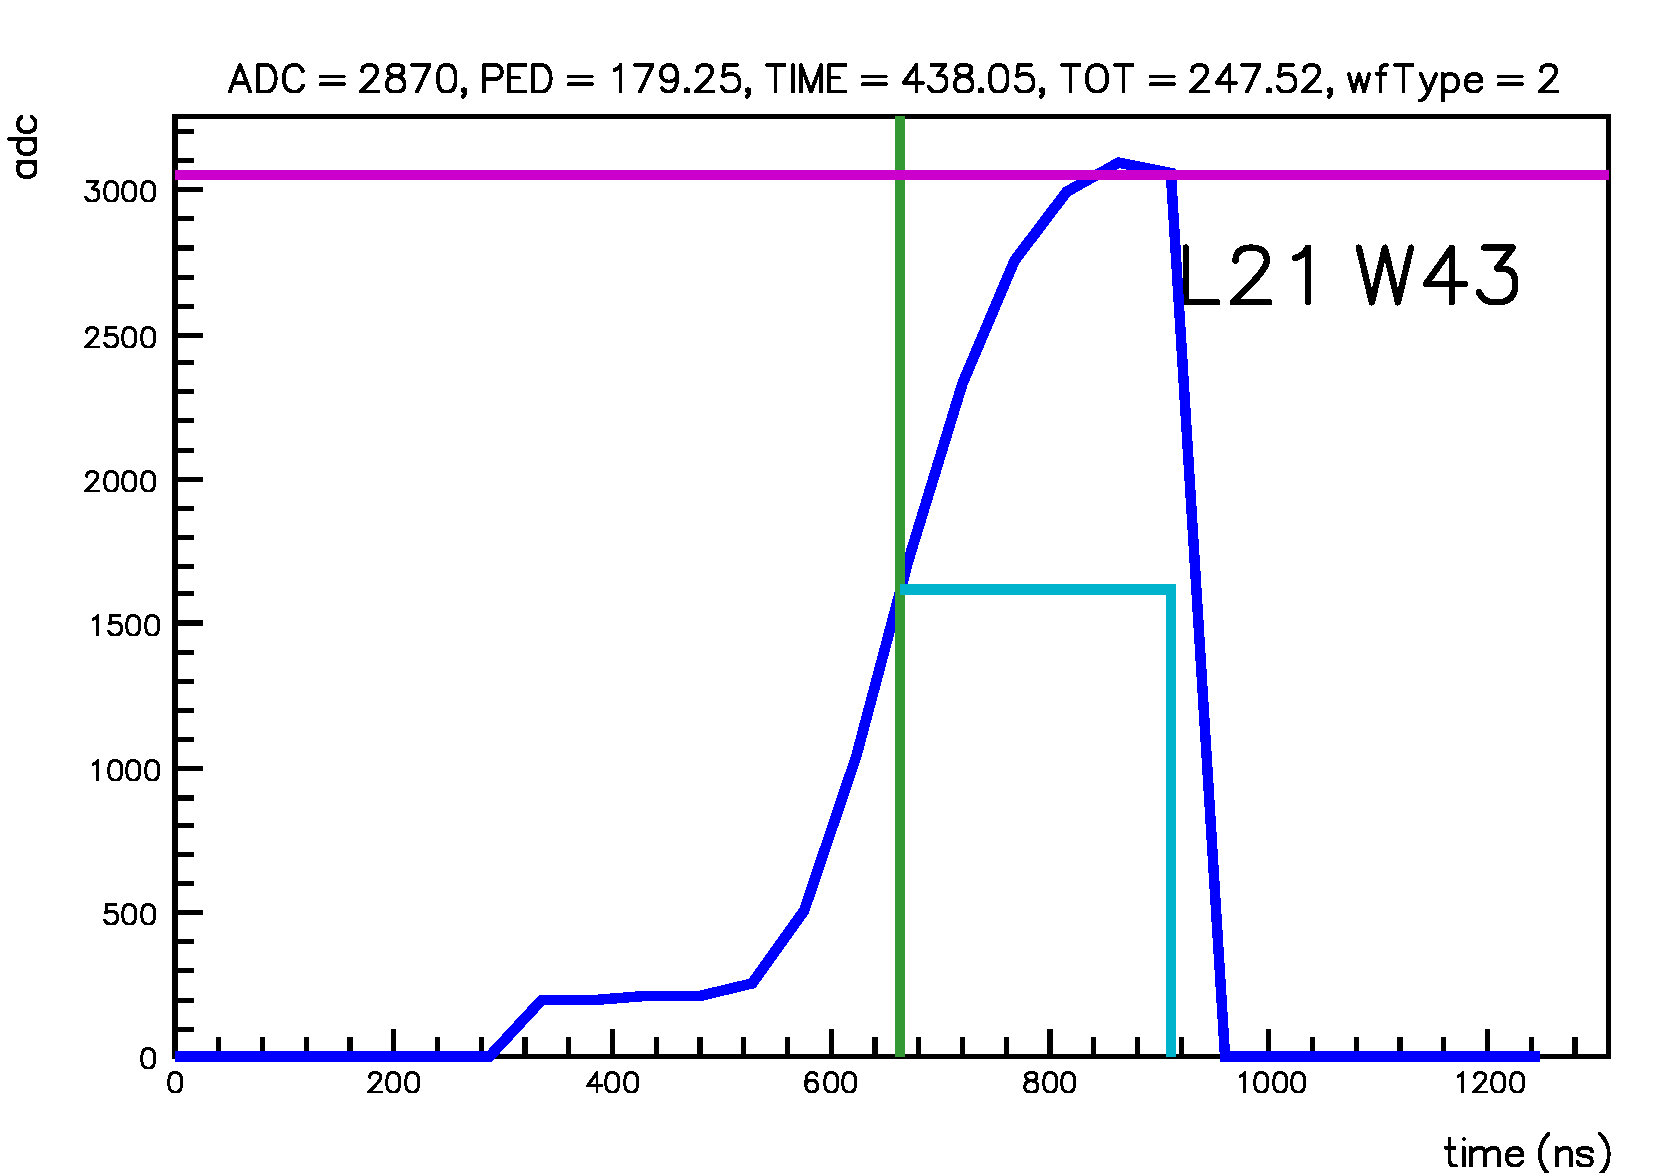
\includegraphics[width=\linewidth]{figures/wf2_after.pdf}

         \centering
        {\color{red} After}
    \end{minipage}


\end{frame}




% \begin{frame}{Fix: Do not the ToT cut for wfType 1 and 2}
%     \begin{itemize}
%         \item \textbf{Bug:} In p0v12, I applied ToT cut on wfType 1 (saturated signals) and wfType 2 (missing trailing edge) while their ToT is bad defined
%         \item Below is a fix
%     \end{itemize}


%     \vspace{0.3cm}
%     \centering
%     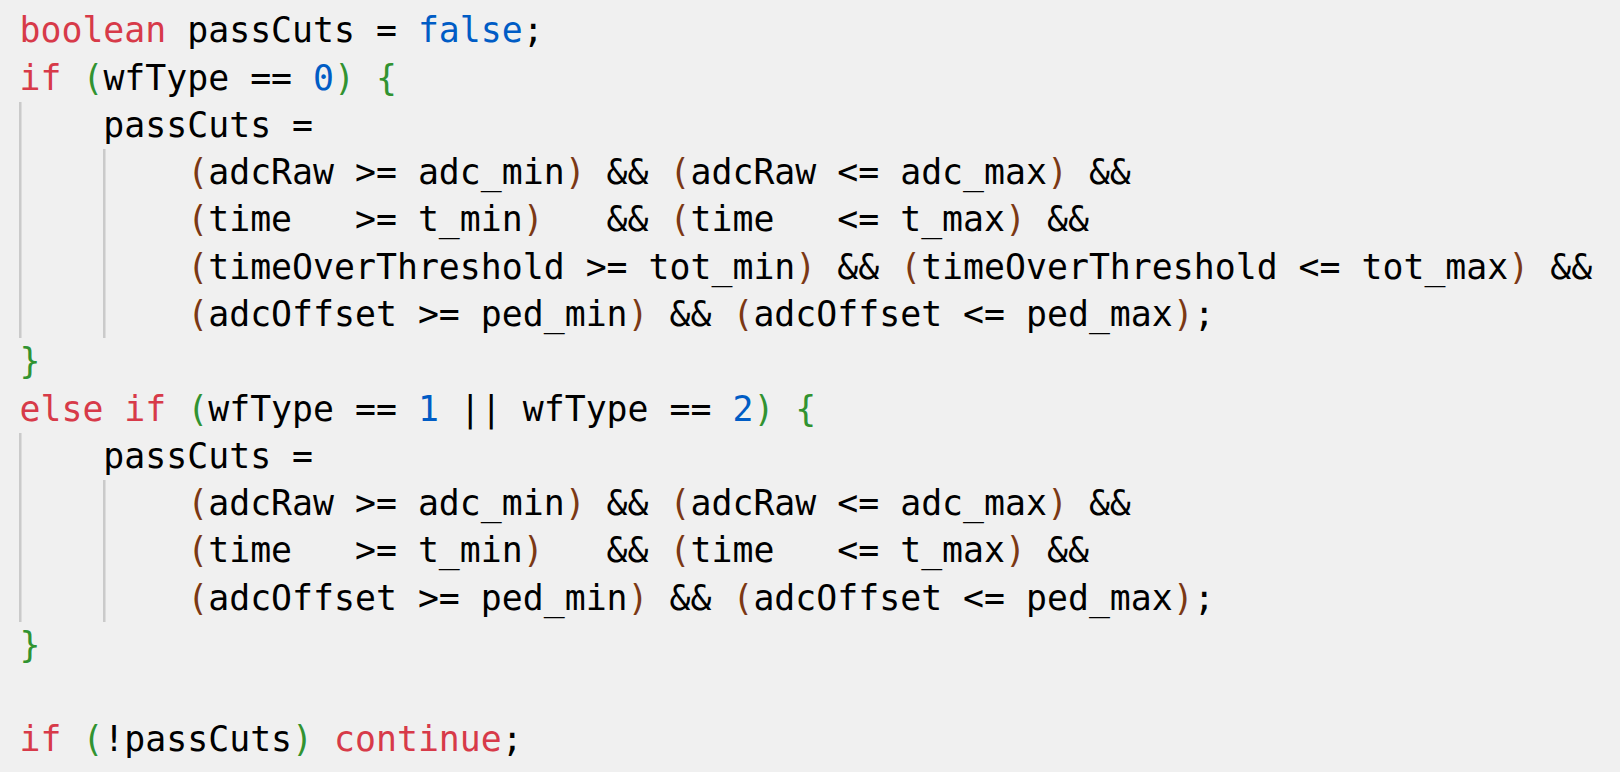
\includegraphics[width=0.6\linewidth]{figures/passCuts.png}



% \end{frame}

\begin{frame}{Effect on the reconstruction}
    \begin{itemize}
        \item I was not expecting a big change, as most of these waveforms seem to be out of time.
        \item This correction has a small effect on the data
        \item I earned 1 \% of elastic events
        \item Run 22772, $^4$He, 2.24 GeV 
    \end{itemize}

    \begin{tabular}{cc}
        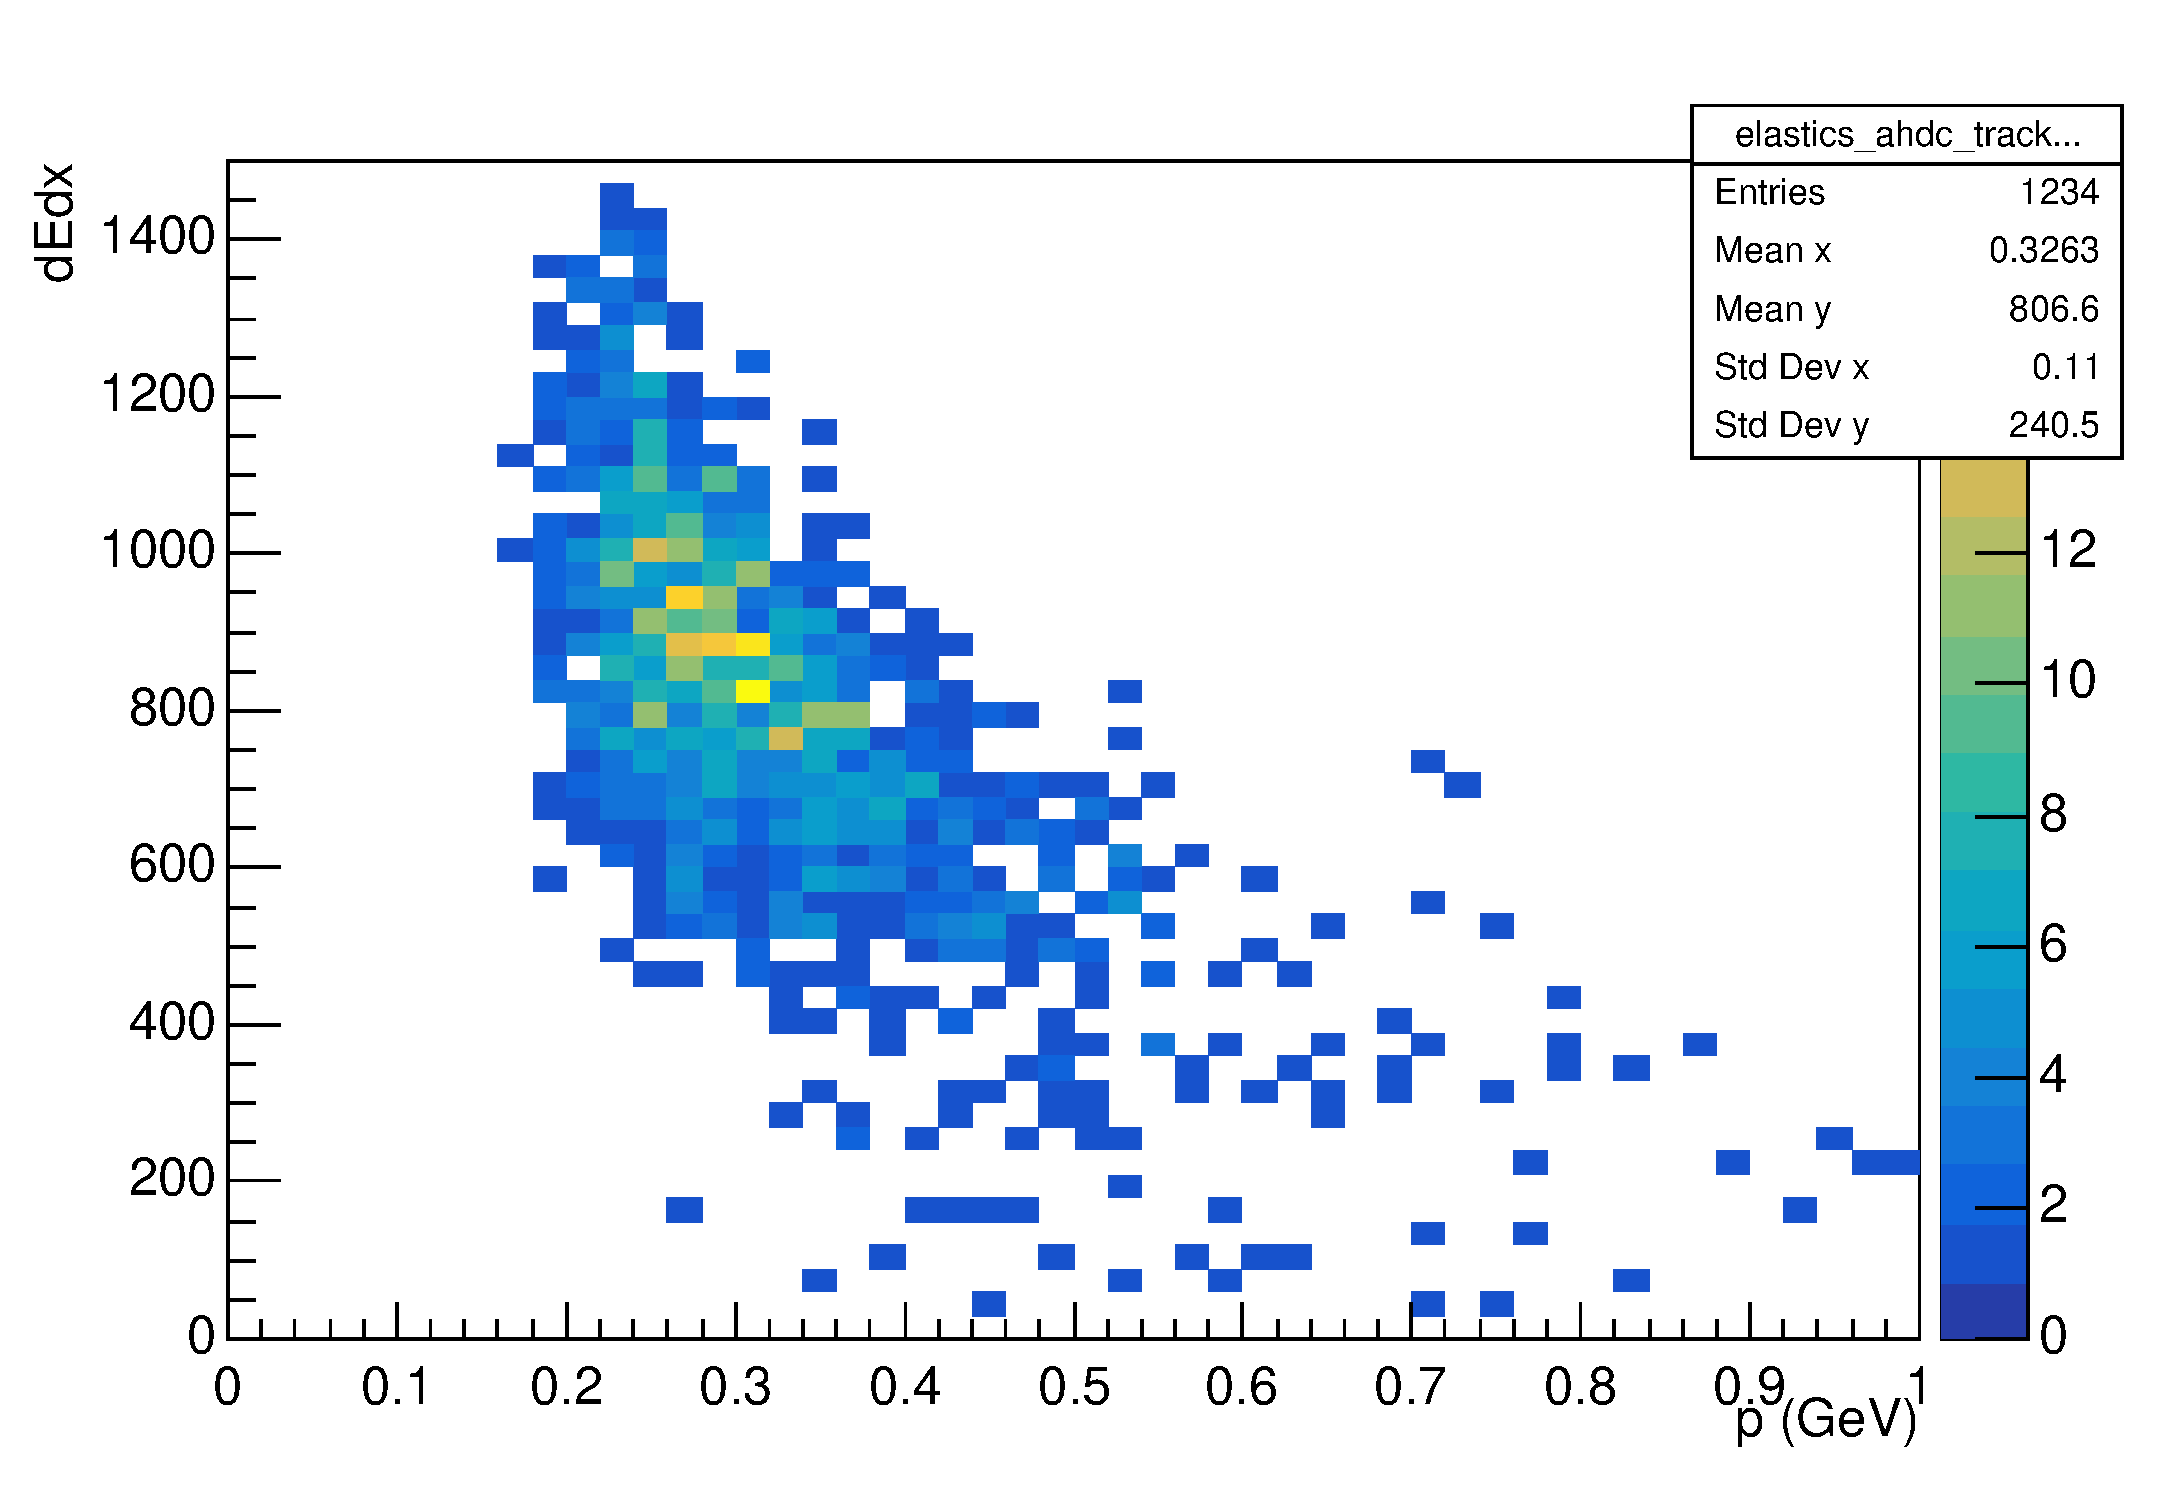
\includegraphics[width=0.45\textwidth]{figures/old_dEdx_vs_p.pdf} & 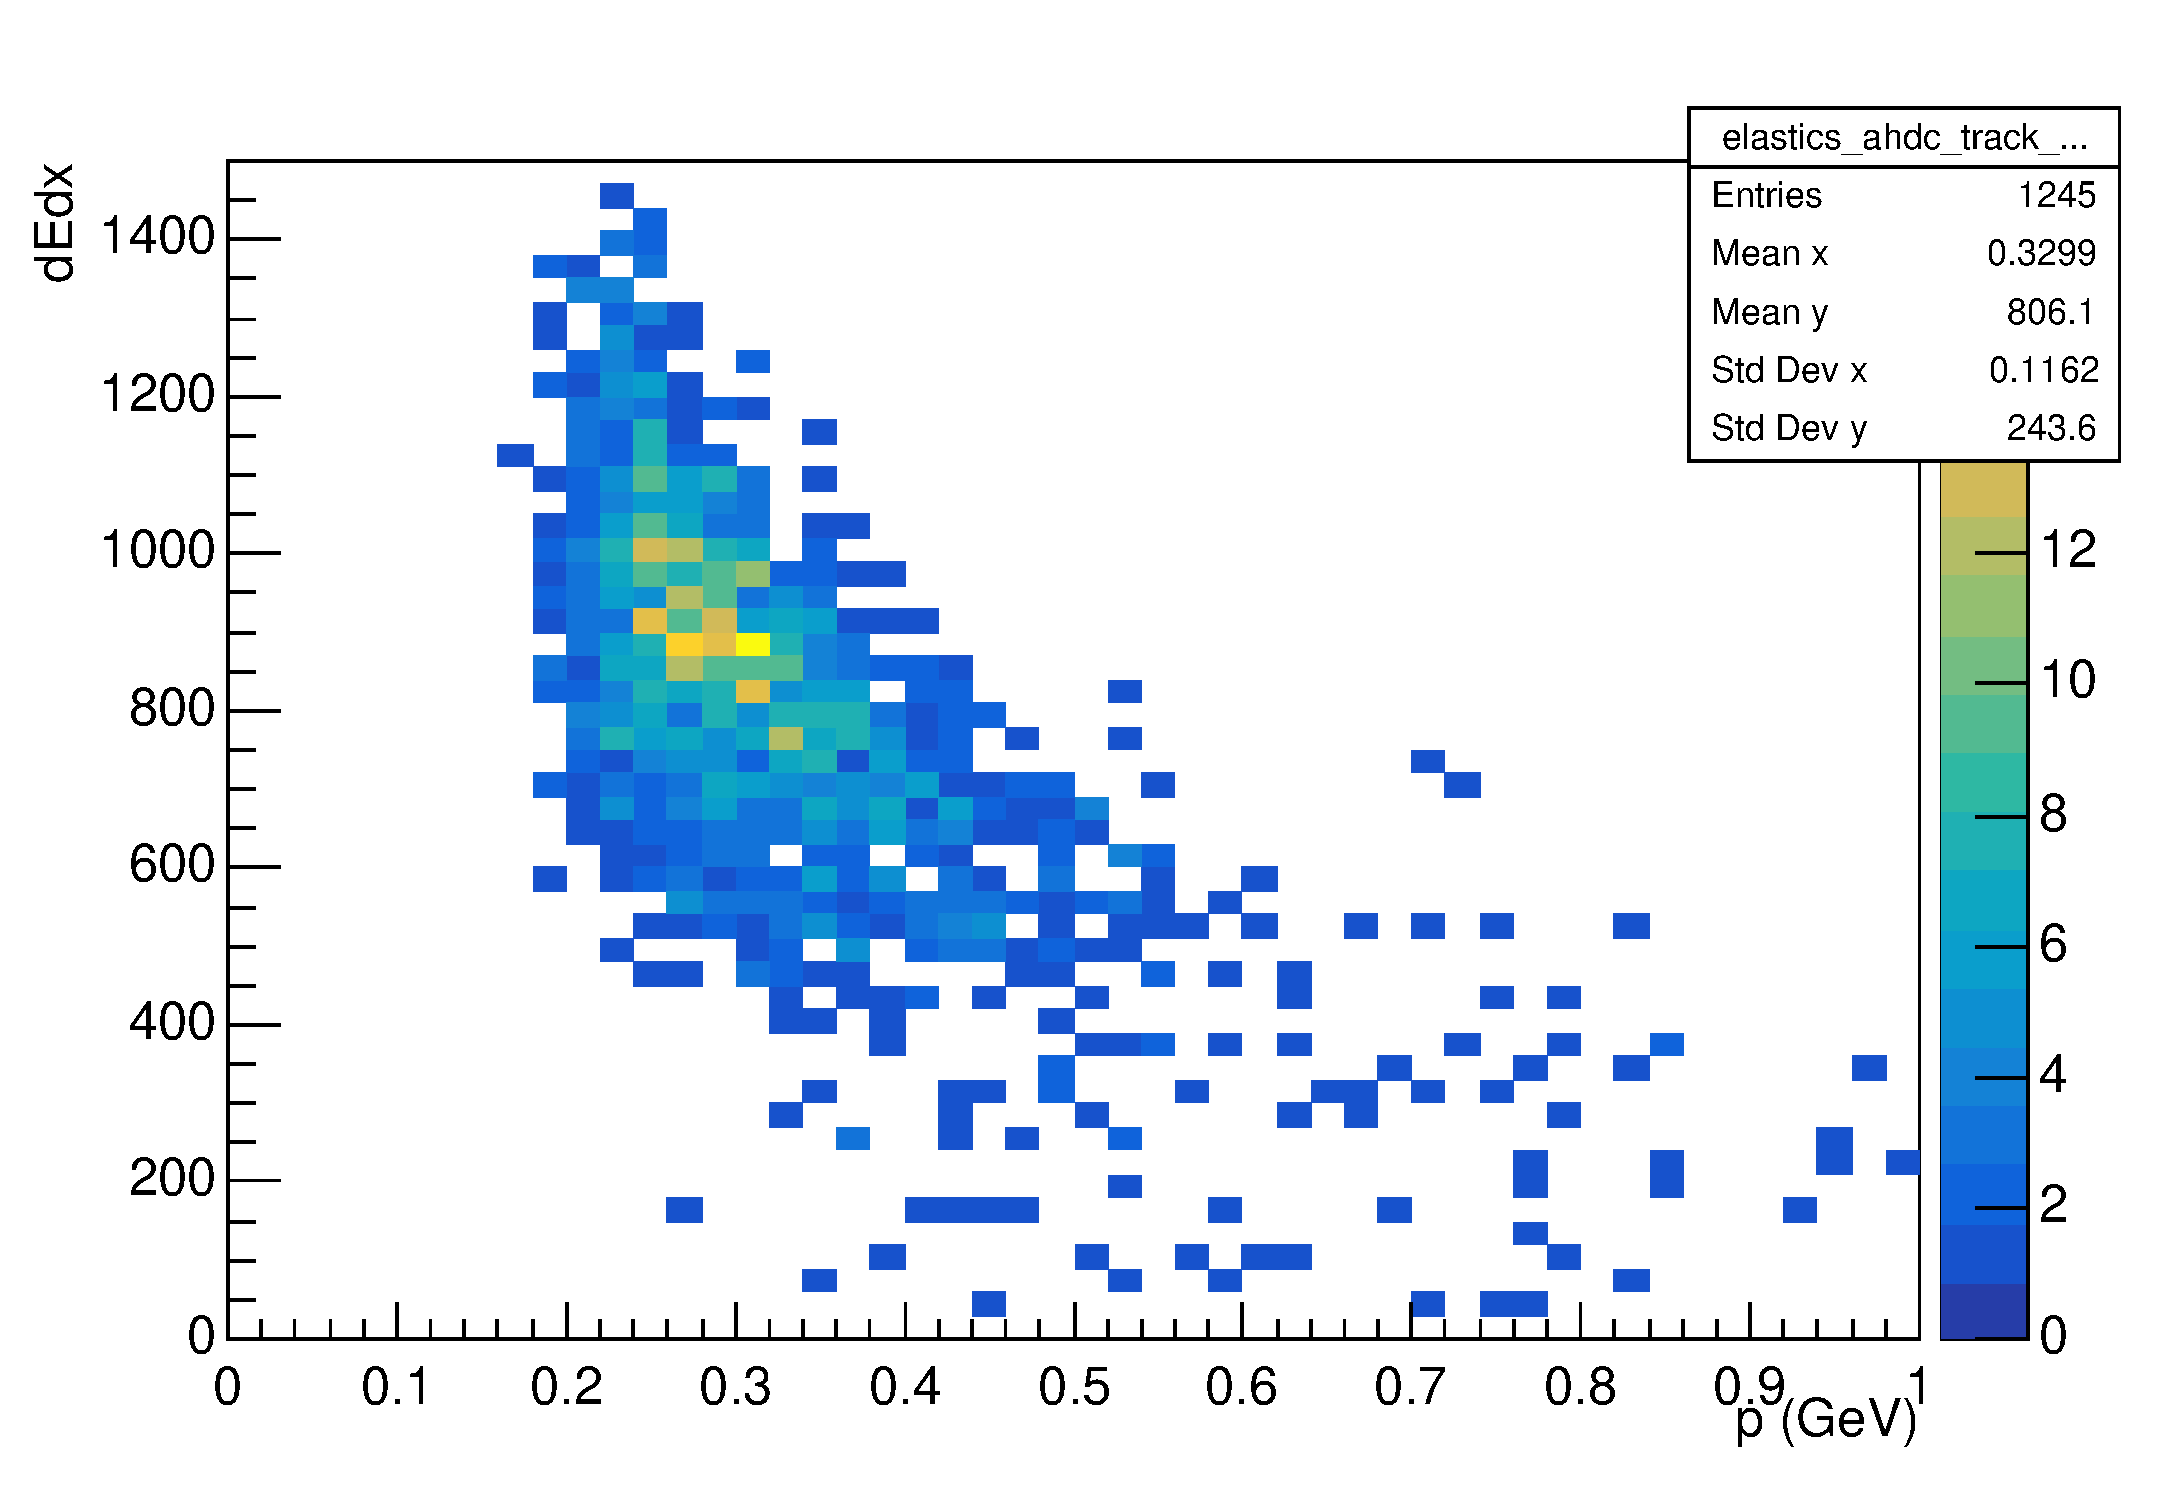
\includegraphics[width=0.45\textwidth]{figures/new_dEdx_vs_p.pdf}
    \end{tabular}

    \begin{itemize}
        \item I will submit a pull request in the coming days.
    \end{itemize}
    
\end{frame}


% \begin{frame}{Illustration of the ToT cut for wfType 1}

%     \begin{itemize}
%         \item Example on run 22172, 4He, 10.6 GeV, 325 nA
%         \item Here I was expecting to reconstruct the track with the big deposited energy
%         \item Actually, the hits did not pass the selection cuts because I was requiring ToT $<$ 300 ns while they are saturated
%         \item {\color{red} Changer l'illustration, utiliser la version de amon-gui où le temps affiché est le celui calibré}
%         % \item Instead, I reconstructed an artifact (magenta circles)
%         %     \begin{itemize}
%         %         \item Most of the saturated hits may seem late, I just think they need their own t0 calibration (what is not done yet)
%         %         \item Their ToT do not really make sense, and I should have removed the cut on the ToT for these signals
%         %     \end{itemize}
%     \end{itemize}

%     \begin{minipage}{0.4\textwidth}
%         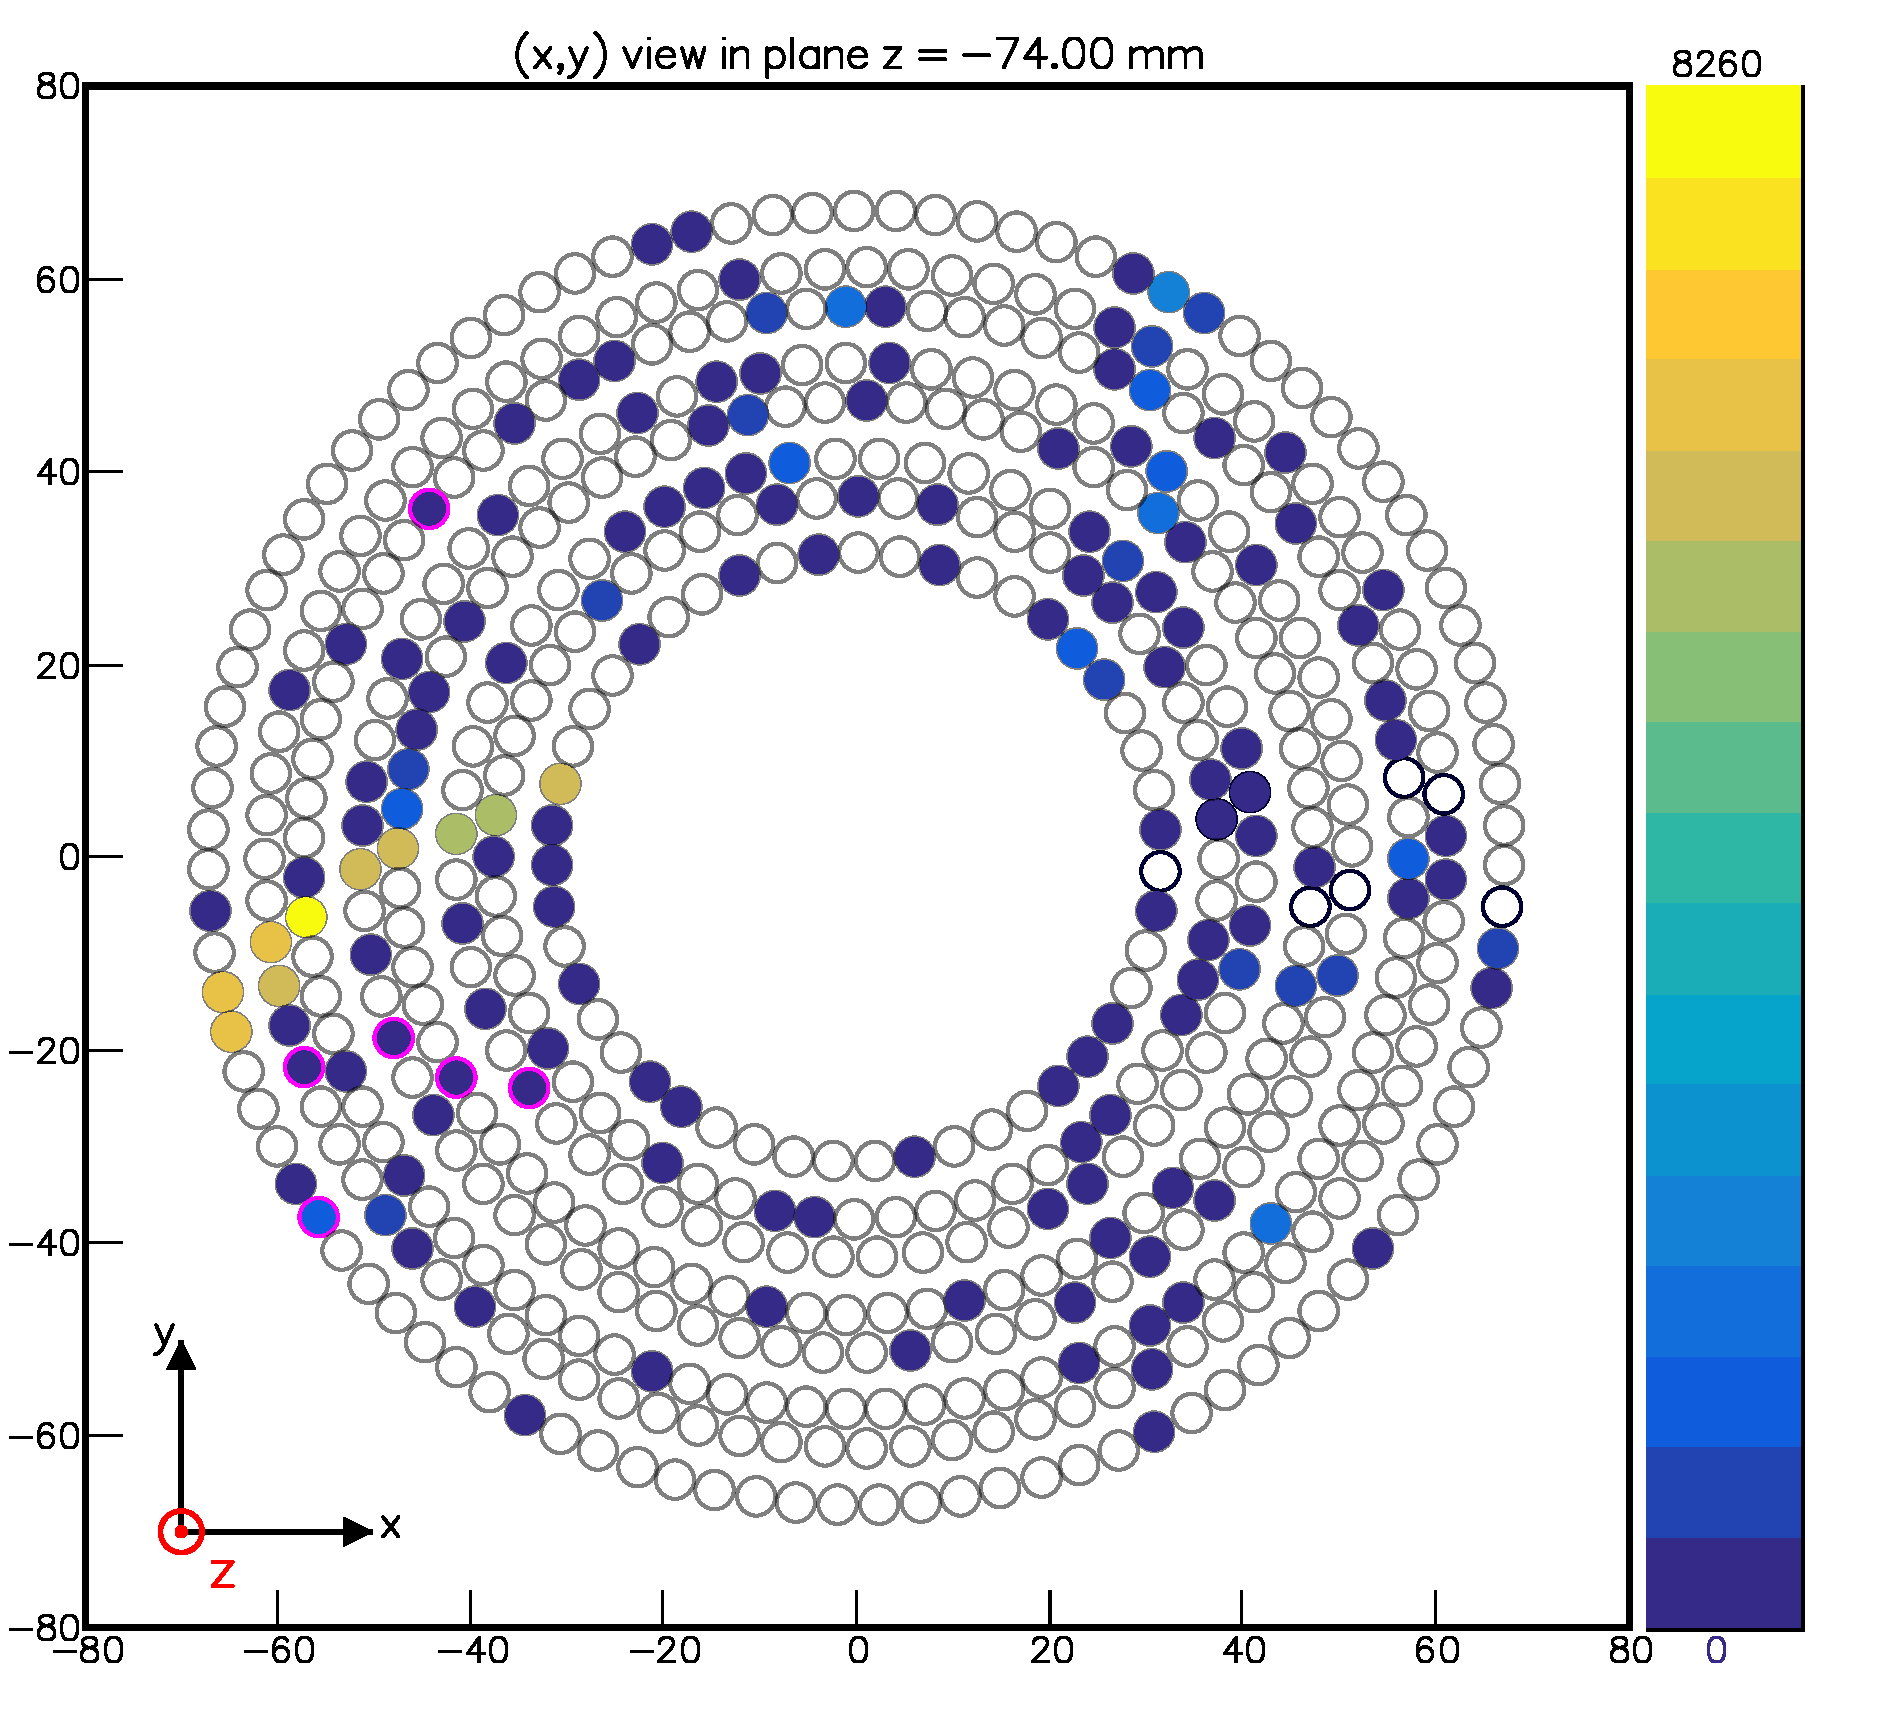
\includegraphics[width=\linewidth]{figures/issue_with_helium_run_num_1.pdf}
%     \end{minipage}
%     \begin{minipage}{0.58\textwidth}
%         \begin{tabular}{cc}
%             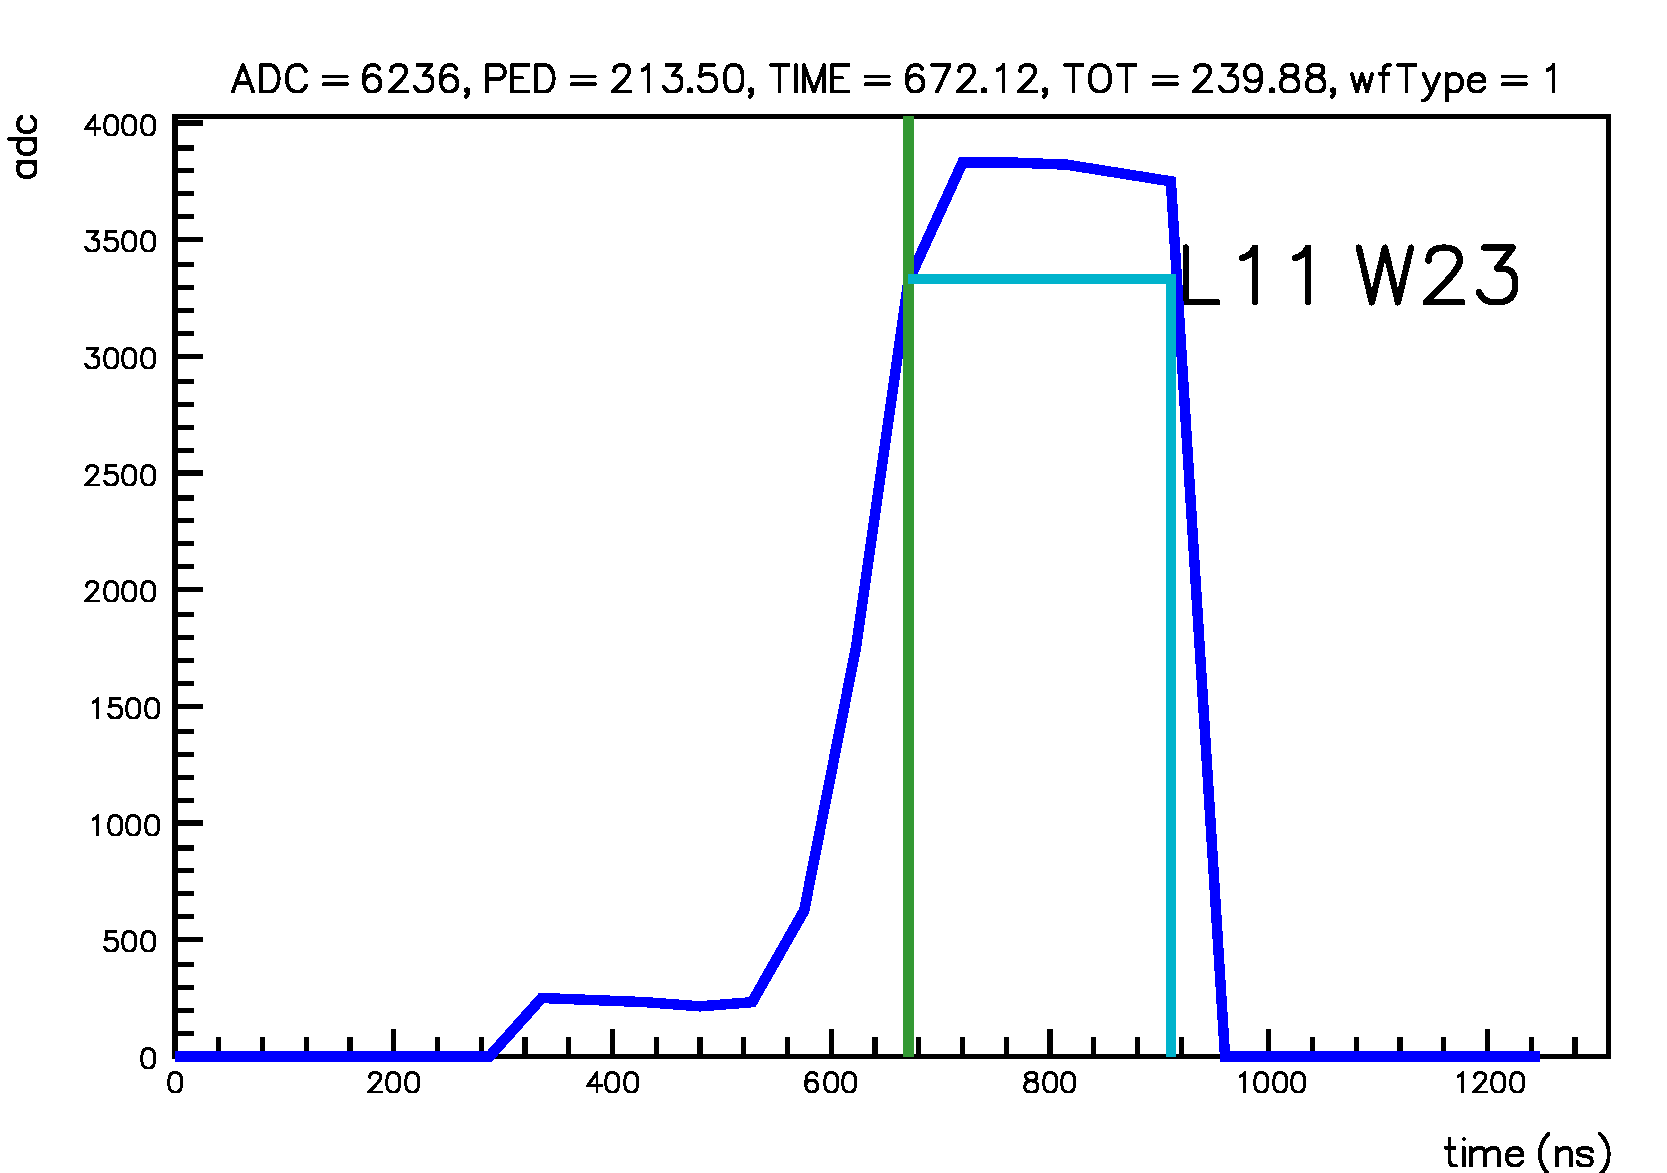
\includegraphics[width=0.45\textwidth]{figures/issue_with_helium_run_num_1_wf1.pdf} &
%                 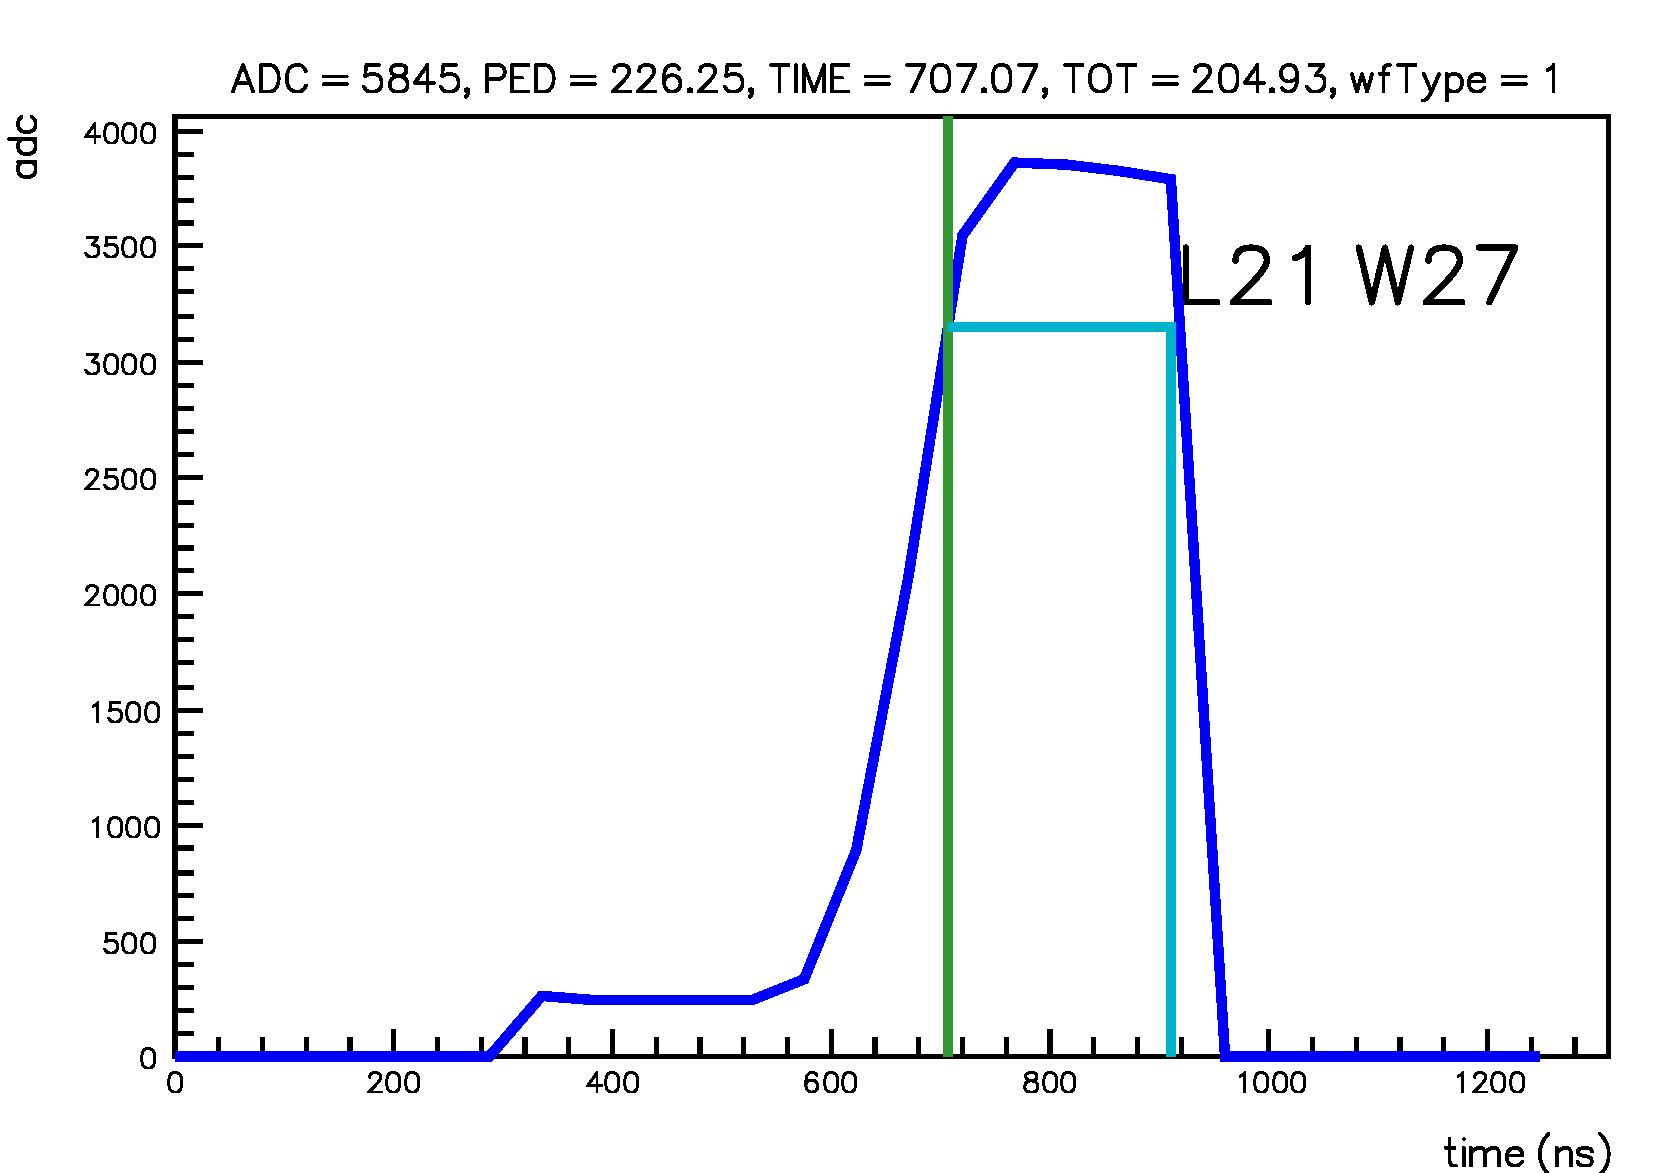
\includegraphics[width=0.45\textwidth]{figures/issue_with_helium_run_num_1_wf2.pdf} \\
%             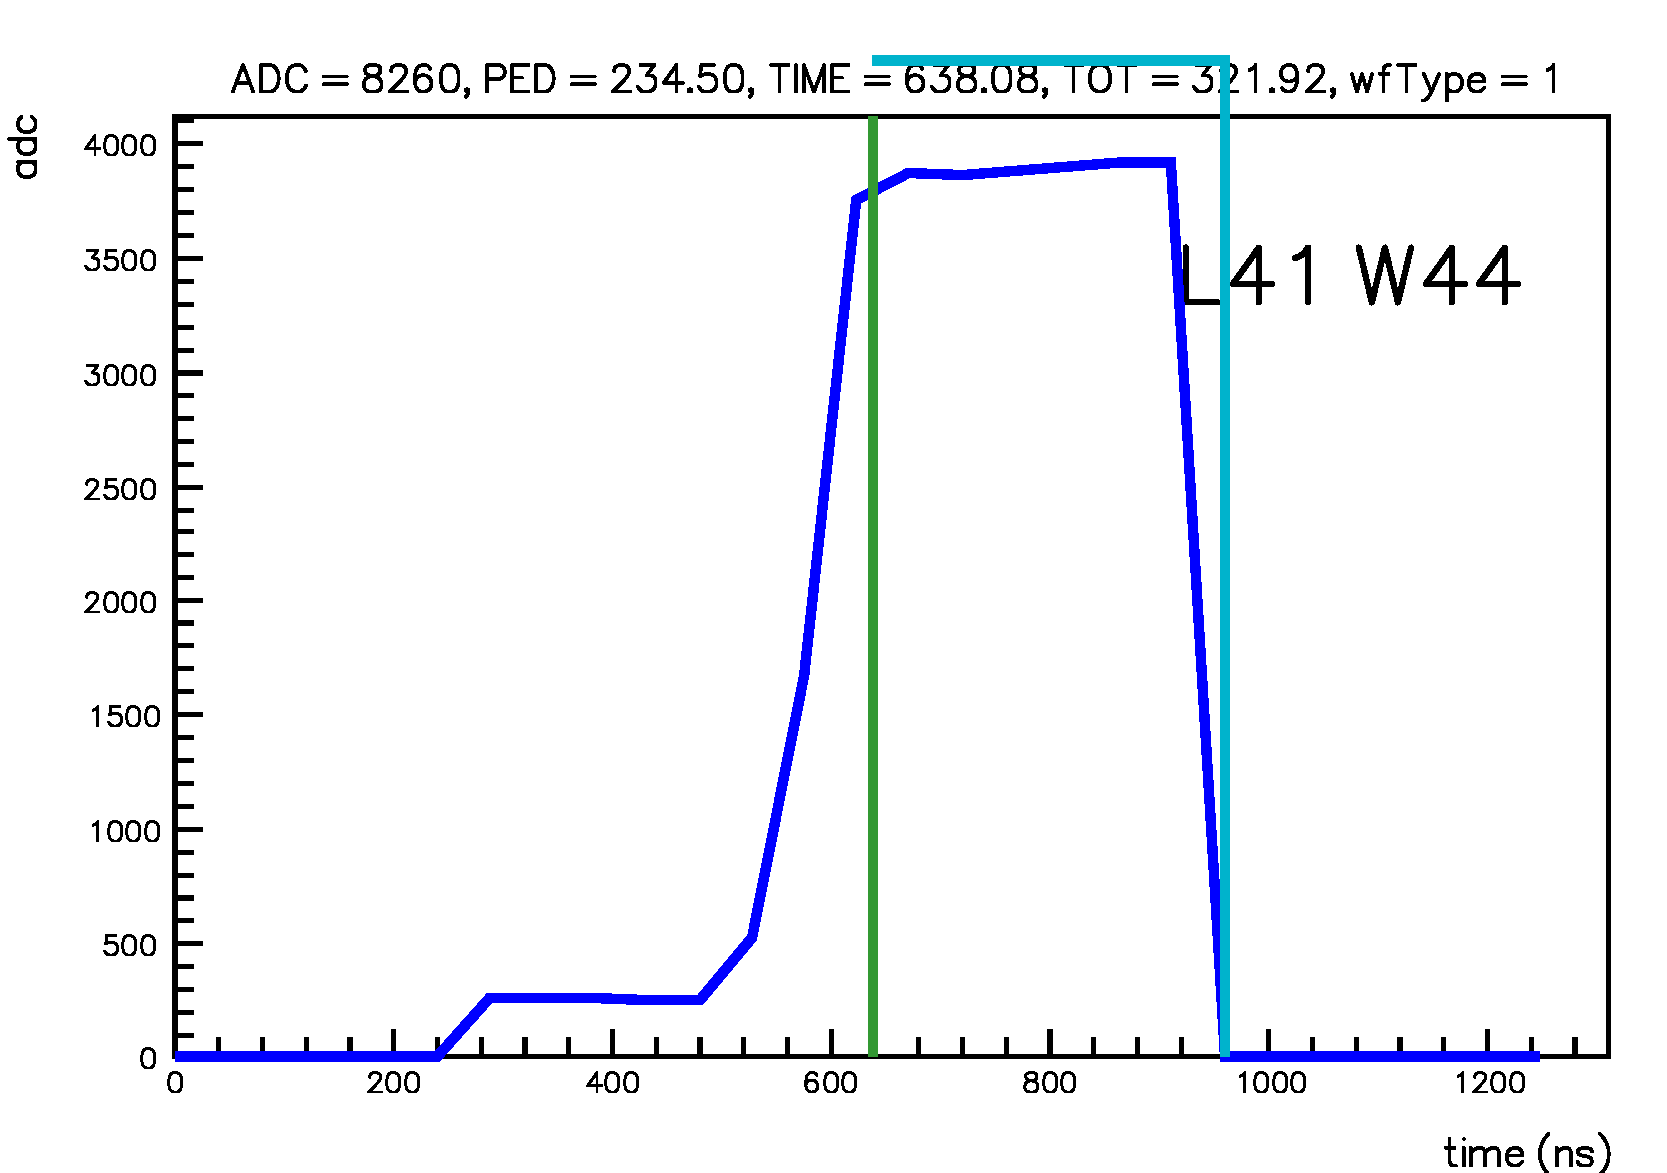
\includegraphics[width=0.45\textwidth]{figures/issue_with_helium_run_num_1_wf3.pdf} &
%                 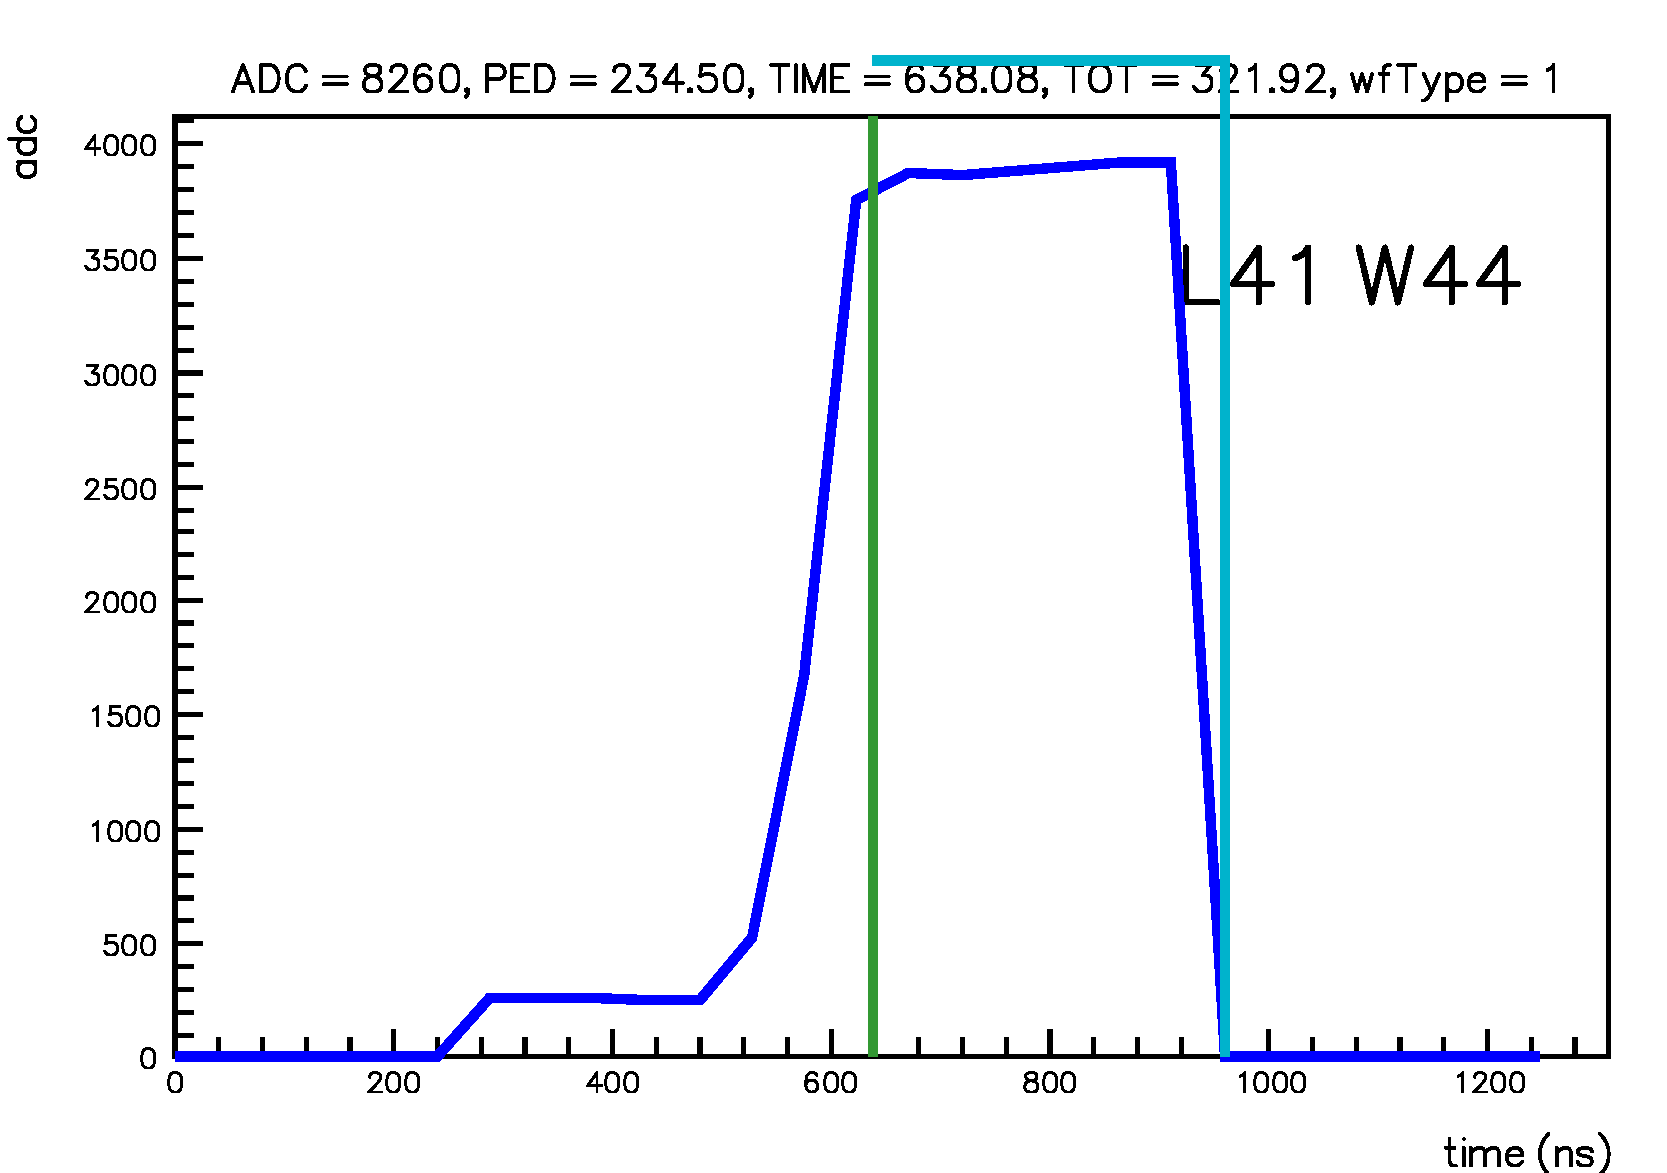
\includegraphics[width=0.45\textwidth]{figures/issue_with_helium_run_num_1_wf3.pdf} \\
%         \end{tabular}
%     \end{minipage}


%     \begin{itemize}
%         \item However, even if they pass the selection cuts, they are out of time (are they really ?)
%     \end{itemize}
    
% \end{frame}


% \begin{frame}{Next steps}
    
%     \begin{itemize}
%         \item 
%     \end{itemize}


    
% \end{frame}

\end{document}


